%---------------------------------------------------------------------
%
%                          Ap�ndice 1
%
%---------------------------------------------------------------------

\chapter{Simulaciones}
\label{apendiceC}

A continuaci�n se incluyen las simulaciones realizadas sobre los procesadores en el siguiente orden:

\begin{enumerate}
  \item Prueba de control sobre procesador est�ndar.
  \item Prueba con fallos sobre procesador est�ndar.
  \item Prueba de control sobre procesador tolerante a fallos.
  \item Prueba con fallos sobre procesador tolerante a fallos.
\end{enumerate}


% Procesador_A 
\newpage
\begin{figure}[ht]
	\section{Procesador est�ndar sin fallos}
	\label{apendiceC:proc}
  \centering

	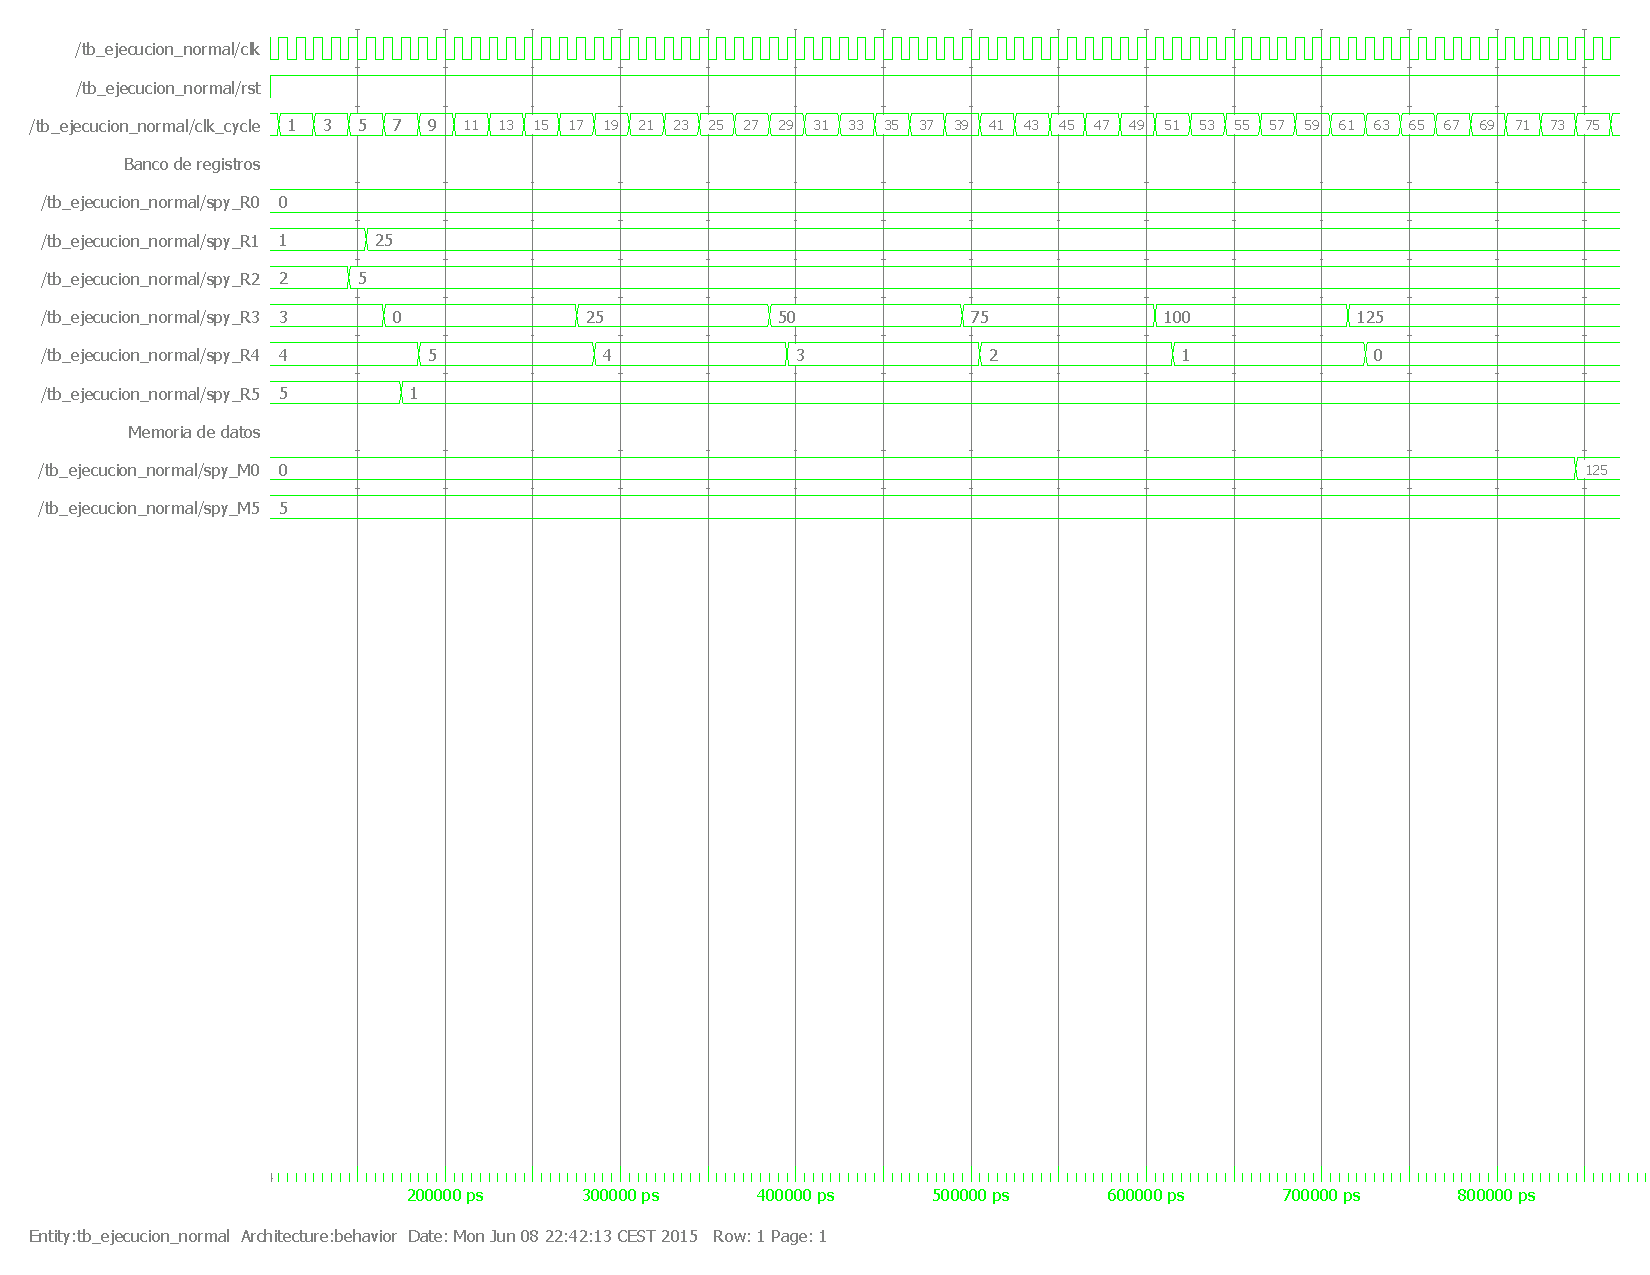
\includepdf[pages=-,scale=.72,pagecommand={},angle=90]{PDFs/Procesador_A.pdf}
	%\includegraphics[width=\textwidth,angle=90]
		%{PDFs/Procesador_A.eps}

\end{figure}

% Procesador_B
\newpage
\begin{figure}[ht]
	\section{Procesador est�ndar con fallos}
	\label{apendiceC:proc:fallos}
  \centering

	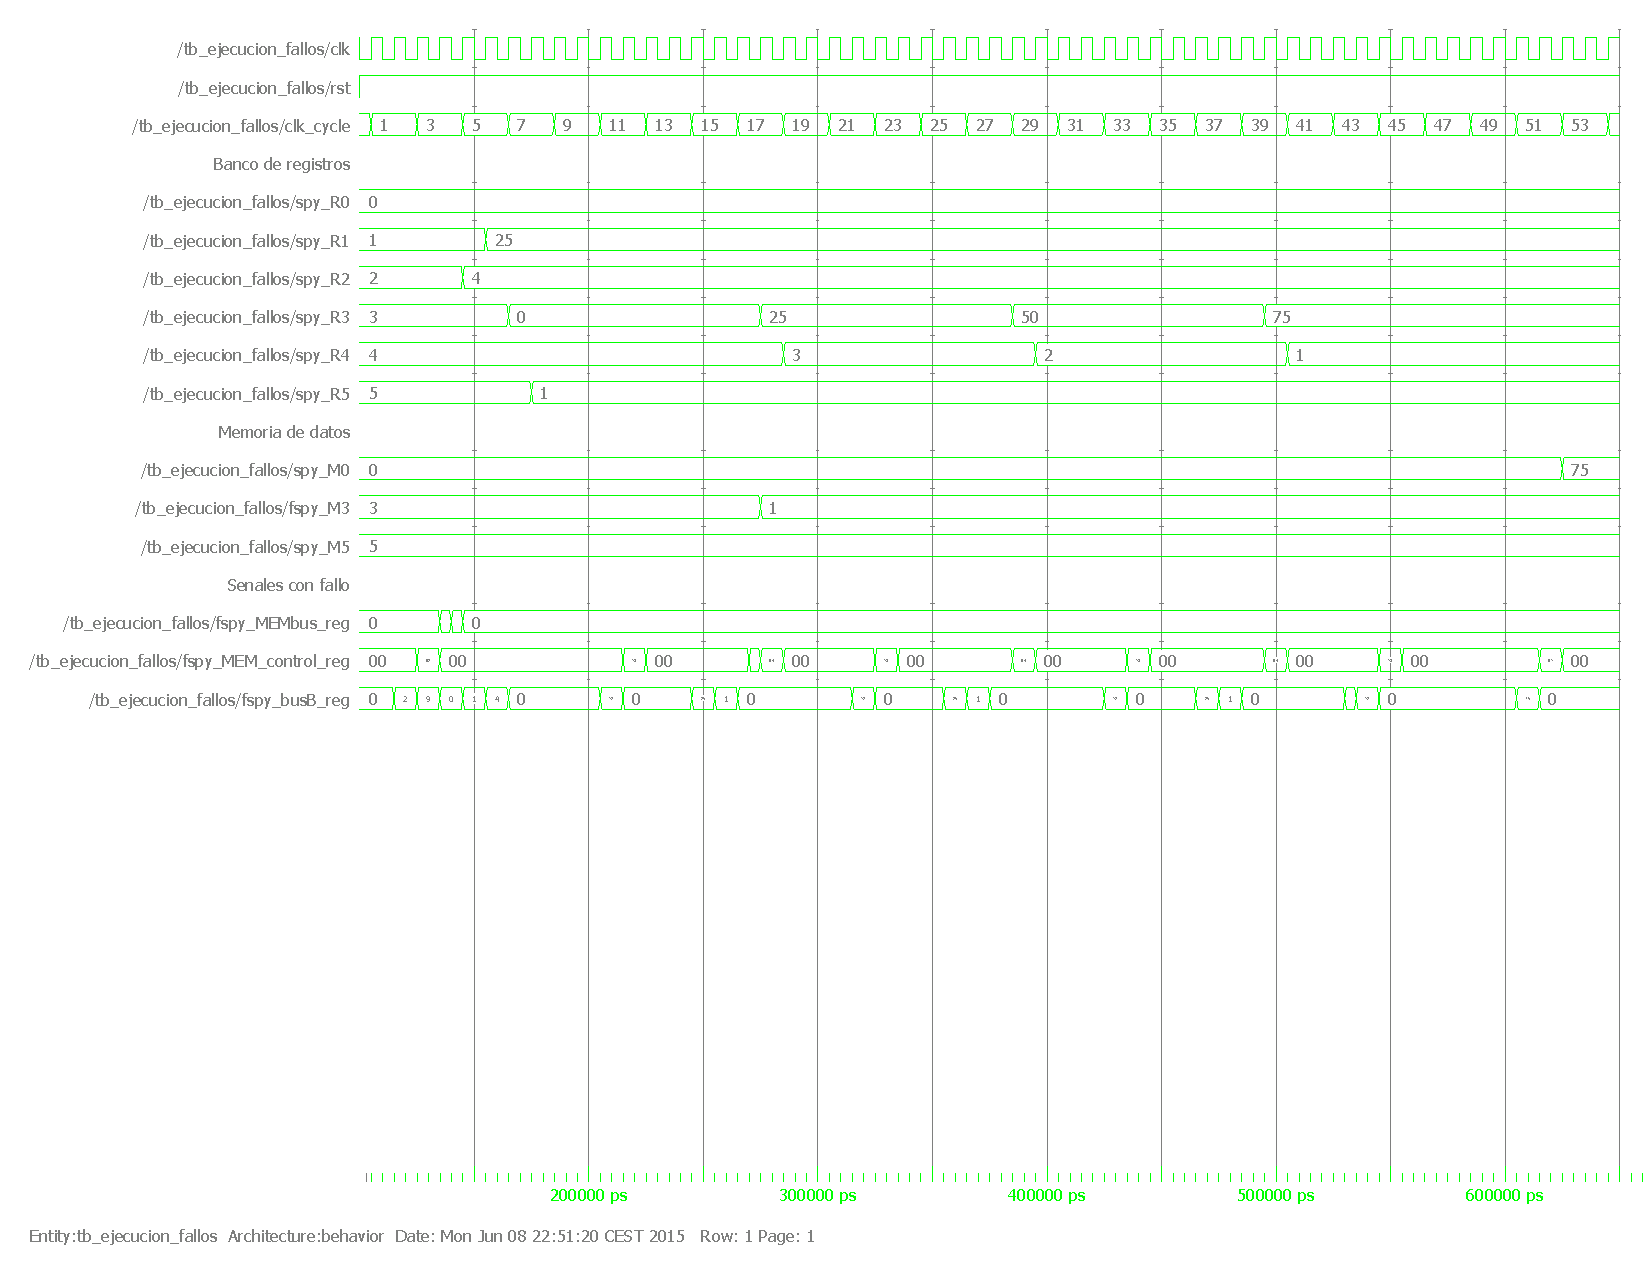
\includepdf[pages=-,scale=.72,pagecommand={},angle=90]
		{PDFs/Procesador_B.pdf}
	%\includegraphics[width=\textwidth,angle=90]
		%{PDFs/Procesador_B.eps}

\end{figure}

% Procesador_TF_A
\newpage
\begin{figure}[ht]
	\section{Procesador tolerante a fallos sin fallos}
	\label{apendiceC:proctf}
  \centering

	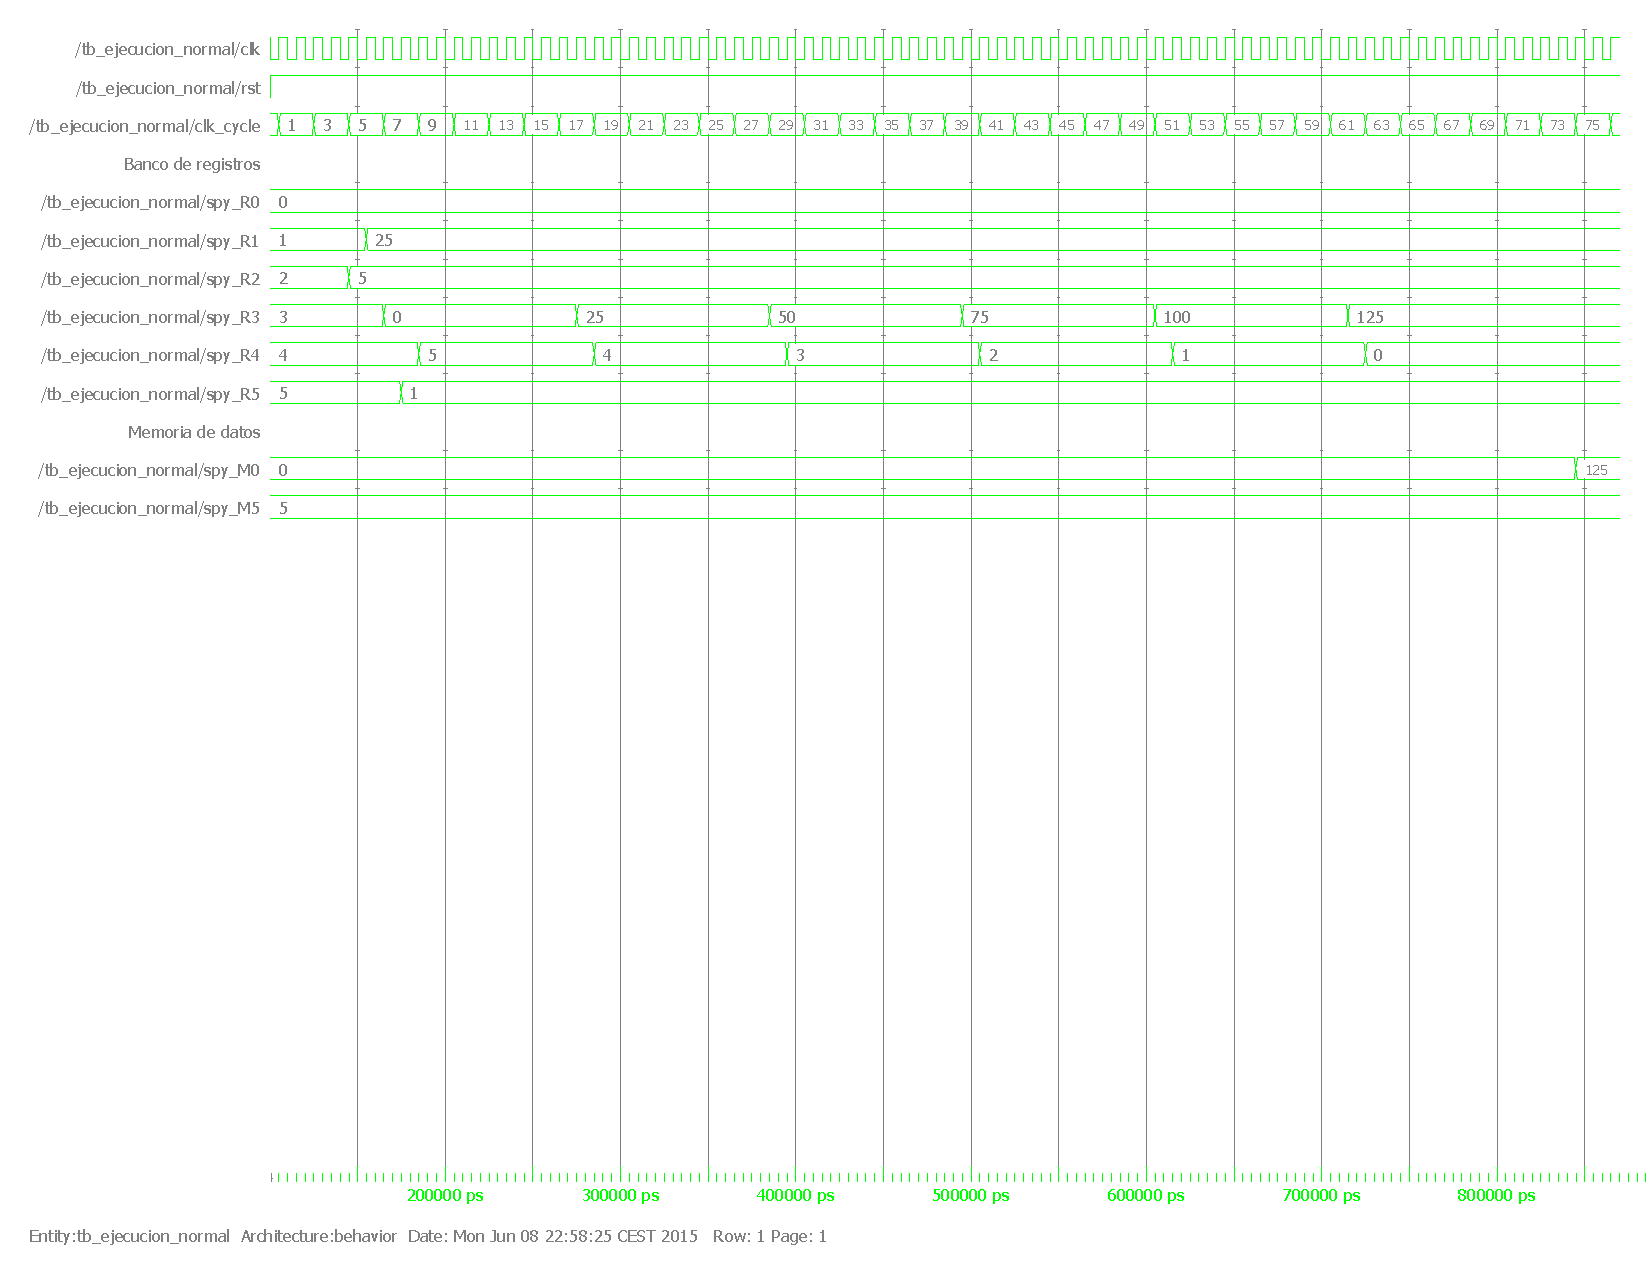
\includepdf[pages=-,scale=.72,pagecommand={},angle=90]
		{PDFs/ProcesadorTF_A.pdf}
	%\includegraphics[width=\textwidth,angle=90]
		%{PDFs/ProcesadorTF_A.eps}

\end{figure}

% Procesador_TF_B
\newpage
\begin{figure}[ht]
	\section{Procesador tolerante a fallos con fallos}
	\label{apendiceC:proctf:fallos}
	\centering

	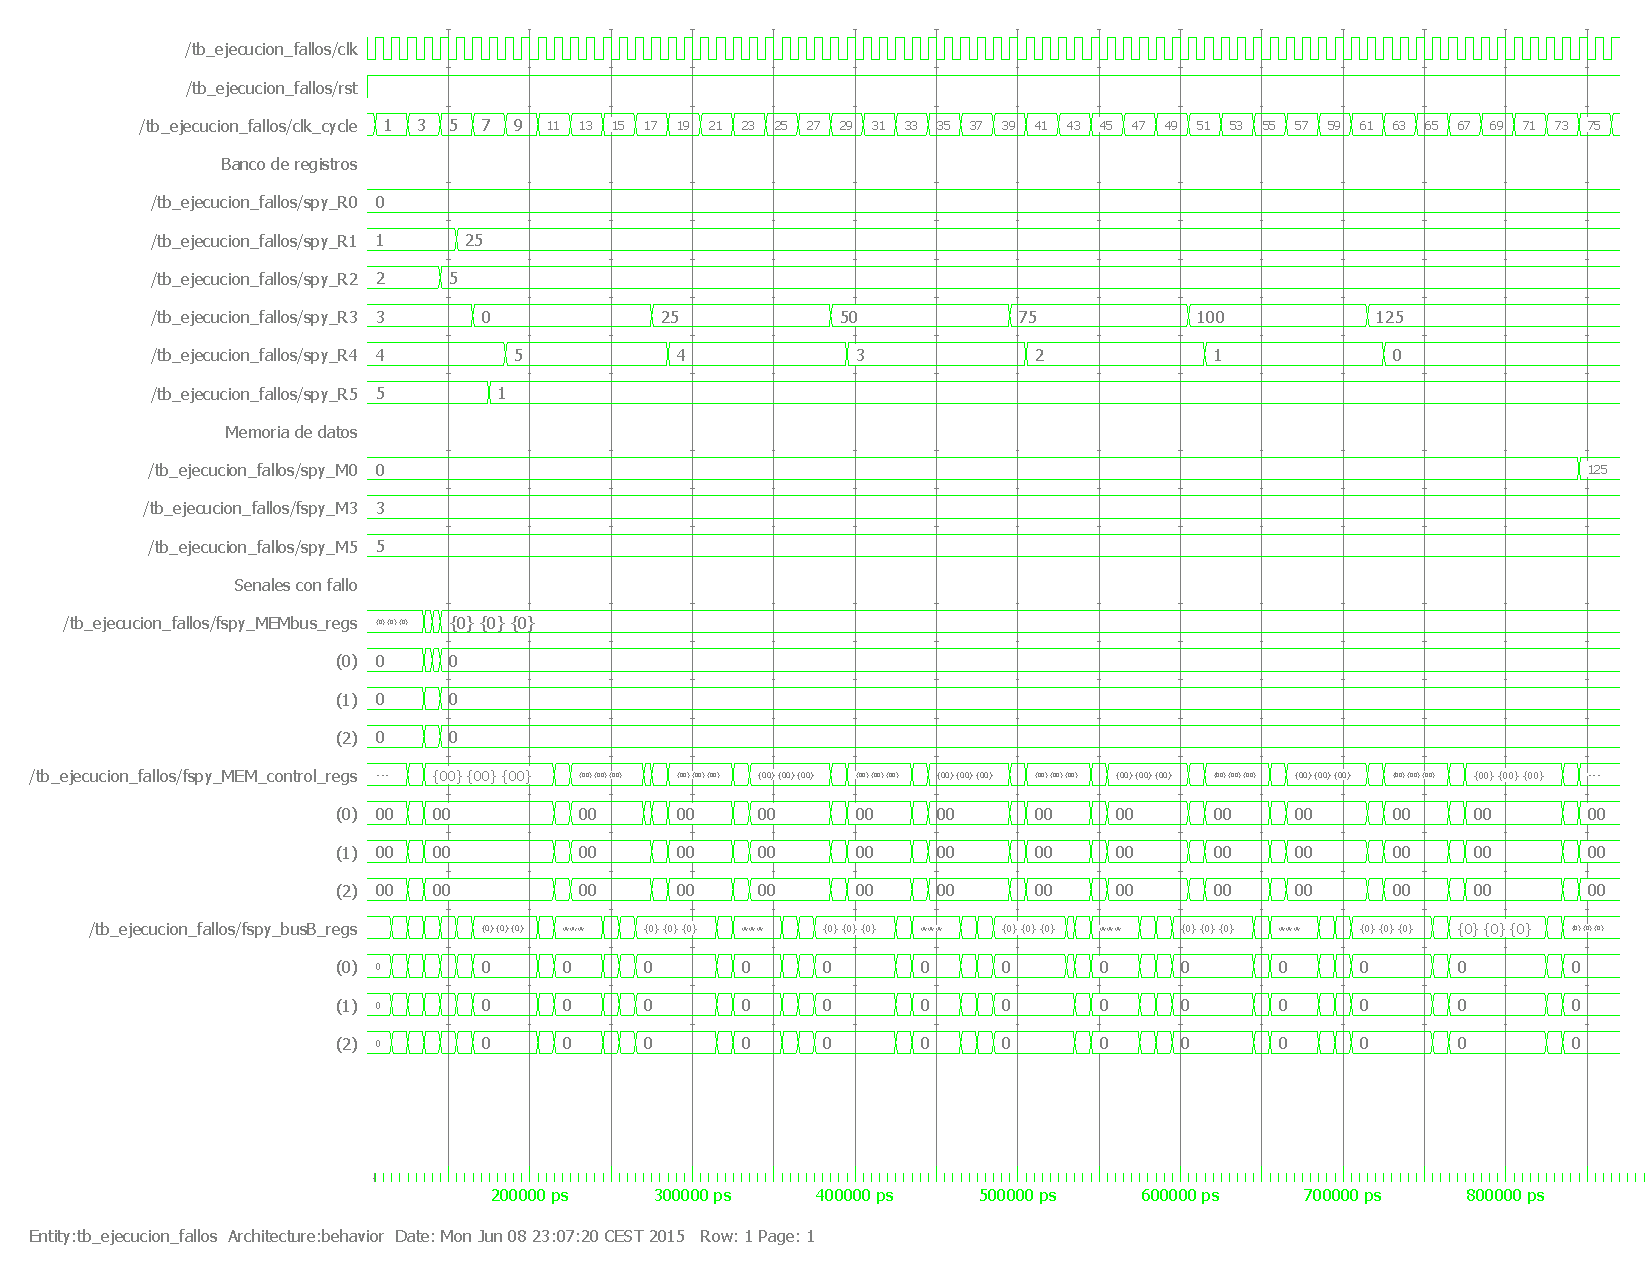
\includepdf[pages=-,scale=.72,pagecommand={},angle=90]
		{PDFs/ProcesadorTF_B.pdf}
	%\includegraphics[width=\textwidth,angle=90]
		%{PDFs/ProcesadorTF_B2.eps}

\end{figure}


